% Options for packages loaded elsewhere
\PassOptionsToPackage{unicode}{hyperref}
\PassOptionsToPackage{hyphens}{url}
\documentclass[
]{article}
\usepackage{xcolor}
\usepackage[margin=1in]{geometry}
\usepackage{amsmath,amssymb}
\setcounter{secnumdepth}{5}
\usepackage{iftex}
\ifPDFTeX
  \usepackage[T1]{fontenc}
  \usepackage[utf8]{inputenc}
  \usepackage{textcomp} % provide euro and other symbols
\else % if luatex or xetex
  \usepackage{unicode-math} % this also loads fontspec
  \defaultfontfeatures{Scale=MatchLowercase}
  \defaultfontfeatures[\rmfamily]{Ligatures=TeX,Scale=1}
\fi
\usepackage{lmodern}
\ifPDFTeX\else
  % xetex/luatex font selection
\fi
% Use upquote if available, for straight quotes in verbatim environments
\IfFileExists{upquote.sty}{\usepackage{upquote}}{}
\IfFileExists{microtype.sty}{% use microtype if available
  \usepackage[]{microtype}
  \UseMicrotypeSet[protrusion]{basicmath} % disable protrusion for tt fonts
}{}
\makeatletter
\@ifundefined{KOMAClassName}{% if non-KOMA class
  \IfFileExists{parskip.sty}{%
    \usepackage{parskip}
  }{% else
    \setlength{\parindent}{0pt}
    \setlength{\parskip}{6pt plus 2pt minus 1pt}}
}{% if KOMA class
  \KOMAoptions{parskip=half}}
\makeatother
\usepackage{color}
\usepackage{fancyvrb}
\newcommand{\VerbBar}{|}
\newcommand{\VERB}{\Verb[commandchars=\\\{\}]}
\DefineVerbatimEnvironment{Highlighting}{Verbatim}{commandchars=\\\{\}}
% Add ',fontsize=\small' for more characters per line
\usepackage{framed}
\definecolor{shadecolor}{RGB}{248,248,248}
\newenvironment{Shaded}{\begin{snugshade}}{\end{snugshade}}
\newcommand{\AlertTok}[1]{\textcolor[rgb]{0.94,0.16,0.16}{#1}}
\newcommand{\AnnotationTok}[1]{\textcolor[rgb]{0.56,0.35,0.01}{\textbf{\textit{#1}}}}
\newcommand{\AttributeTok}[1]{\textcolor[rgb]{0.13,0.29,0.53}{#1}}
\newcommand{\BaseNTok}[1]{\textcolor[rgb]{0.00,0.00,0.81}{#1}}
\newcommand{\BuiltInTok}[1]{#1}
\newcommand{\CharTok}[1]{\textcolor[rgb]{0.31,0.60,0.02}{#1}}
\newcommand{\CommentTok}[1]{\textcolor[rgb]{0.56,0.35,0.01}{\textit{#1}}}
\newcommand{\CommentVarTok}[1]{\textcolor[rgb]{0.56,0.35,0.01}{\textbf{\textit{#1}}}}
\newcommand{\ConstantTok}[1]{\textcolor[rgb]{0.56,0.35,0.01}{#1}}
\newcommand{\ControlFlowTok}[1]{\textcolor[rgb]{0.13,0.29,0.53}{\textbf{#1}}}
\newcommand{\DataTypeTok}[1]{\textcolor[rgb]{0.13,0.29,0.53}{#1}}
\newcommand{\DecValTok}[1]{\textcolor[rgb]{0.00,0.00,0.81}{#1}}
\newcommand{\DocumentationTok}[1]{\textcolor[rgb]{0.56,0.35,0.01}{\textbf{\textit{#1}}}}
\newcommand{\ErrorTok}[1]{\textcolor[rgb]{0.64,0.00,0.00}{\textbf{#1}}}
\newcommand{\ExtensionTok}[1]{#1}
\newcommand{\FloatTok}[1]{\textcolor[rgb]{0.00,0.00,0.81}{#1}}
\newcommand{\FunctionTok}[1]{\textcolor[rgb]{0.13,0.29,0.53}{\textbf{#1}}}
\newcommand{\ImportTok}[1]{#1}
\newcommand{\InformationTok}[1]{\textcolor[rgb]{0.56,0.35,0.01}{\textbf{\textit{#1}}}}
\newcommand{\KeywordTok}[1]{\textcolor[rgb]{0.13,0.29,0.53}{\textbf{#1}}}
\newcommand{\NormalTok}[1]{#1}
\newcommand{\OperatorTok}[1]{\textcolor[rgb]{0.81,0.36,0.00}{\textbf{#1}}}
\newcommand{\OtherTok}[1]{\textcolor[rgb]{0.56,0.35,0.01}{#1}}
\newcommand{\PreprocessorTok}[1]{\textcolor[rgb]{0.56,0.35,0.01}{\textit{#1}}}
\newcommand{\RegionMarkerTok}[1]{#1}
\newcommand{\SpecialCharTok}[1]{\textcolor[rgb]{0.81,0.36,0.00}{\textbf{#1}}}
\newcommand{\SpecialStringTok}[1]{\textcolor[rgb]{0.31,0.60,0.02}{#1}}
\newcommand{\StringTok}[1]{\textcolor[rgb]{0.31,0.60,0.02}{#1}}
\newcommand{\VariableTok}[1]{\textcolor[rgb]{0.00,0.00,0.00}{#1}}
\newcommand{\VerbatimStringTok}[1]{\textcolor[rgb]{0.31,0.60,0.02}{#1}}
\newcommand{\WarningTok}[1]{\textcolor[rgb]{0.56,0.35,0.01}{\textbf{\textit{#1}}}}
\usepackage{longtable,booktabs,array}
\usepackage{calc} % for calculating minipage widths
% Correct order of tables after \paragraph or \subparagraph
\usepackage{etoolbox}
\makeatletter
\patchcmd\longtable{\par}{\if@noskipsec\mbox{}\fi\par}{}{}
\makeatother
% Allow footnotes in longtable head/foot
\IfFileExists{footnotehyper.sty}{\usepackage{footnotehyper}}{\usepackage{footnote}}
\makesavenoteenv{longtable}
\usepackage{graphicx}
\makeatletter
\newsavebox\pandoc@box
\newcommand*\pandocbounded[1]{% scales image to fit in text height/width
  \sbox\pandoc@box{#1}%
  \Gscale@div\@tempa{\textheight}{\dimexpr\ht\pandoc@box+\dp\pandoc@box\relax}%
  \Gscale@div\@tempb{\linewidth}{\wd\pandoc@box}%
  \ifdim\@tempb\p@<\@tempa\p@\let\@tempa\@tempb\fi% select the smaller of both
  \ifdim\@tempa\p@<\p@\scalebox{\@tempa}{\usebox\pandoc@box}%
  \else\usebox{\pandoc@box}%
  \fi%
}
% Set default figure placement to htbp
\def\fps@figure{htbp}
\makeatother
\setlength{\emergencystretch}{3em} % prevent overfull lines
\providecommand{\tightlist}{%
  \setlength{\itemsep}{0pt}\setlength{\parskip}{0pt}}
\usepackage[]{natbib}
\bibliographystyle{plainnat}
\usepackage{bookmark}
\IfFileExists{xurl.sty}{\usepackage{xurl}}{} % add URL line breaks if available
\urlstyle{same}
\hypersetup{
  pdftitle={Appendix C --- Nonlinear Modeling of Chess Rating Growth},
  pdfauthor={Tina Huynh},
  hidelinks,
  pdfcreator={LaTeX via pandoc}}

\title{Appendix C --- Nonlinear Modeling of Chess Rating Growth}
\author{Tina Huynh}
\date{2025-10-16}

\begin{document}
\maketitle

{
\setcounter{tocdepth}{2}
\tableofcontents
}
\subsection{Appendix C --- Nonlinear Modeling of Chess Rating
Growth}\label{appendix-c-nonlinear-modeling-of-chess-rating-growth}

\subsubsection{C.1 Conceptual Overview}\label{c.1-conceptual-overview}

Linear mixed-effects models assume rating growth is constant over time
--- but human learning typically follows an \textbf{asymptotic curve}: -
Rapid improvement early on (steep initial slope) - Gradual slowdown as
players approach their skill ceiling

We model this using a \textbf{logistic growth function} or an
\textbf{exponential saturation model}.

\[
R_t = A - B \times e^{-k t}
\]

where: - \(R_t\): Rating at time \(t\) - \(A\): Asymptotic rating
ceiling - \(B\): Range between starting and ceiling rating - \(k\):
Learning rate constant

\begin{center}\rule{0.5\linewidth}{0.5pt}\end{center}

\subsubsection{C.2 Model Preparation}\label{c.2-model-preparation}

\begin{Shaded}
\begin{Highlighting}[]
\FunctionTok{library}\NormalTok{(tidyverse)}
\FunctionTok{library}\NormalTok{(broom)}
\FunctionTok{library}\NormalTok{(minpack.lm) }\CommentTok{\# for nlsLM (robust nonlinear fitting)}

\NormalTok{rating\_history\_path }\OtherTok{\textless{}{-}} \StringTok{"../../data/lichess\_rating\_history.csv"}

\CommentTok{\# Load the same dataset from Appendix B}
\NormalTok{rating\_summary }\OtherTok{\textless{}{-}} \FunctionTok{read\_csv}\NormalTok{(}
\NormalTok{  rating\_history\_path,}
  \AttributeTok{show\_col\_types =} \ConstantTok{FALSE}
\NormalTok{)}

\CommentTok{\# Filter for Blitz category for consistency}
\NormalTok{rating\_nl\_df }\OtherTok{\textless{}{-}}\NormalTok{ rating\_summary }\SpecialCharTok{\%\textgreater{}\%}
  \FunctionTok{filter}\NormalTok{(category }\SpecialCharTok{==} \StringTok{"Blitz"}\NormalTok{, }\SpecialCharTok{!}\FunctionTok{is.na}\NormalTok{(rating)) }\SpecialCharTok{\%\textgreater{}\%}
  \FunctionTok{group\_by}\NormalTok{(user) }\SpecialCharTok{\%\textgreater{}\%}
  \FunctionTok{mutate}\NormalTok{(}
    \AttributeTok{time\_index =} \FunctionTok{as.numeric}\NormalTok{(}\FunctionTok{factor}\NormalTok{(}\FunctionTok{row\_number}\NormalTok{())),}
    \AttributeTok{time\_scaled =}\NormalTok{ time\_index }\SpecialCharTok{/} \FunctionTok{max}\NormalTok{(time\_index)}
\NormalTok{  ) }\SpecialCharTok{\%\textgreater{}\%}
  \FunctionTok{filter}\NormalTok{(}\FunctionTok{n}\NormalTok{() }\SpecialCharTok{\textgreater{}=} \DecValTok{10}\NormalTok{) }\SpecialCharTok{\%\textgreater{}\%} \CommentTok{\# ensure sufficient data}
  \FunctionTok{ungroup}\NormalTok{()}

\CommentTok{\# Select a few users for model fitting}
\NormalTok{target\_users }\OtherTok{\textless{}{-}}\NormalTok{ rating\_nl\_df }\SpecialCharTok{\%\textgreater{}\%}
  \FunctionTok{count}\NormalTok{(user) }\SpecialCharTok{\%\textgreater{}\%}
  \FunctionTok{arrange}\NormalTok{(}\FunctionTok{desc}\NormalTok{(n)) }\SpecialCharTok{\%\textgreater{}\%}
  \FunctionTok{slice\_head}\NormalTok{(}\AttributeTok{n =} \DecValTok{5}\NormalTok{) }\SpecialCharTok{\%\textgreater{}\%}
  \FunctionTok{pull}\NormalTok{(user)}

\NormalTok{target\_users}
\end{Highlighting}
\end{Shaded}

\begin{verbatim}
## [1] "Magnus_Carlsen" "GothamChess"    "ChessNetwork"   "Anna_Chess"    
## [5] "Hikaru"
\end{verbatim}

\begin{center}\rule{0.5\linewidth}{0.5pt}\end{center}

\subsubsection{C.3 Fit Logistic / Exponential
Models}\label{c.3-fit-logistic-exponential-models}

\begin{Shaded}
\begin{Highlighting}[]
\CommentTok{\# Helper function: Fit logistic model per user}
\NormalTok{fit\_growth\_curve }\OtherTok{\textless{}{-}} \ControlFlowTok{function}\NormalTok{(df) \{}
  \FunctionTok{tryCatch}\NormalTok{(}
\NormalTok{    \{}
\NormalTok{      model }\OtherTok{\textless{}{-}} \FunctionTok{nlsLM}\NormalTok{(}
\NormalTok{        rating }\SpecialCharTok{\textasciitilde{}}\NormalTok{ A }\SpecialCharTok{{-}}\NormalTok{ B }\SpecialCharTok{*} \FunctionTok{exp}\NormalTok{(}\SpecialCharTok{{-}}\NormalTok{k }\SpecialCharTok{*}\NormalTok{ time\_index),}
        \AttributeTok{data =}\NormalTok{ df,}
        \AttributeTok{start =} \FunctionTok{list}\NormalTok{(}\AttributeTok{A =} \FunctionTok{max}\NormalTok{(df}\SpecialCharTok{$}\NormalTok{rating), }\AttributeTok{B =} \FunctionTok{max}\NormalTok{(df}\SpecialCharTok{$}\NormalTok{rating) }\SpecialCharTok{{-}} \FunctionTok{min}\NormalTok{(df}\SpecialCharTok{$}\NormalTok{rating), }\AttributeTok{k =} \FloatTok{0.05}\NormalTok{),}
        \AttributeTok{control =} \FunctionTok{nls.lm.control}\NormalTok{(}\AttributeTok{maxiter =} \DecValTok{100}\NormalTok{)}
\NormalTok{      )}
      \FunctionTok{tidy}\NormalTok{(model) }\SpecialCharTok{\%\textgreater{}\%} \FunctionTok{mutate}\NormalTok{(}\AttributeTok{user =} \FunctionTok{unique}\NormalTok{(df}\SpecialCharTok{$}\NormalTok{user))}
\NormalTok{    \},}
    \AttributeTok{error =} \ControlFlowTok{function}\NormalTok{(e) }\ConstantTok{NULL}
\NormalTok{  )}
\NormalTok{\}}

\CommentTok{\# Fit for each user}
\NormalTok{nonlinear\_models }\OtherTok{\textless{}{-}}\NormalTok{ rating\_nl\_df }\SpecialCharTok{\%\textgreater{}\%}
  \FunctionTok{filter}\NormalTok{(user }\SpecialCharTok{\%in\%}\NormalTok{ target\_users) }\SpecialCharTok{\%\textgreater{}\%}
  \FunctionTok{group\_by}\NormalTok{(user) }\SpecialCharTok{\%\textgreater{}\%}
  \FunctionTok{group\_modify}\NormalTok{(}\SpecialCharTok{\textasciitilde{}} \FunctionTok{fit\_growth\_curve}\NormalTok{(.x)) }\SpecialCharTok{\%\textgreater{}\%}
  \FunctionTok{ungroup}\NormalTok{()}
\end{Highlighting}
\end{Shaded}

\begin{verbatim}
## Warning: There was 1 warning in `mutate()`.
## i In argument: `user = unique(df$user)`.
## Caused by warning:
## ! Unknown or uninitialised column: `user`.
## There was 1 warning in `mutate()`.
## i In argument: `user = unique(df$user)`.
## Caused by warning:
## ! Unknown or uninitialised column: `user`.
## There was 1 warning in `mutate()`.
## i In argument: `user = unique(df$user)`.
## Caused by warning:
## ! Unknown or uninitialised column: `user`.
## There was 1 warning in `mutate()`.
## i In argument: `user = unique(df$user)`.
## Caused by warning:
## ! Unknown or uninitialised column: `user`.
## There was 1 warning in `mutate()`.
## i In argument: `user = unique(df$user)`.
## Caused by warning:
## ! Unknown or uninitialised column: `user`.
\end{verbatim}

\begin{Shaded}
\begin{Highlighting}[]
\NormalTok{nonlinear\_models}
\end{Highlighting}
\end{Shaded}

\begin{verbatim}
## # A tibble: 15 x 6
##    user           term  estimate std.error statistic p.value
##    <chr>          <chr>    <dbl>     <dbl>     <dbl>   <dbl>
##  1 Anna_Chess     A      2.42e+3   8.96e+2   2.70    0.00945
##  2 Anna_Chess     B      8.39e+2   8.87e+2   0.946   0.349  
##  3 Anna_Chess     k      6.19e-3   7.81e-3   0.793   0.432  
##  4 ChessNetwork   A     -3.12e+4   2.29e+7  -0.00136 0.999  
##  5 ChessNetwork   B     -3.27e+4   2.29e+7  -0.00143 0.999  
##  6 ChessNetwork   k      4.16e-5   2.91e-2   0.00143 0.999  
##  7 GothamChess    A     -6.59e+3   5.36e+4  -0.123   0.903  
##  8 GothamChess    B     -8.24e+3   5.36e+4  -0.154   0.878  
##  9 GothamChess    k      5.74e-4   3.81e-3   0.150   0.881  
## 10 Hikaru         A      2.74e+4   4.84e+6   0.00565 0.996  
## 11 Hikaru         B      2.57e+4   4.84e+6   0.00531 0.996  
## 12 Hikaru         k     -1.15e-4   2.16e-2  -0.00532 0.996  
## 13 Magnus_Carlsen A      6.61e+4   4.63e+7   0.00143 0.999  
## 14 Magnus_Carlsen B      6.45e+4   4.63e+7   0.00139 0.999  
## 15 Magnus_Carlsen k      2.09e-5   1.50e-2   0.00139 0.999
\end{verbatim}

\begin{center}\rule{0.5\linewidth}{0.5pt}\end{center}

\subsubsection{C.4 Visualization: Fitted Curves vs.~Actual
Data}\label{c.4-visualization-fitted-curves-vs.-actual-data}

\begin{Shaded}
\begin{Highlighting}[]
\NormalTok{predicted\_curves }\OtherTok{\textless{}{-}}\NormalTok{ nonlinear\_models }\SpecialCharTok{\%\textgreater{}\%}
  \FunctionTok{select}\NormalTok{(user, term, estimate) }\SpecialCharTok{\%\textgreater{}\%}
  \FunctionTok{pivot\_wider}\NormalTok{(}\AttributeTok{names\_from =}\NormalTok{ term, }\AttributeTok{values\_from =}\NormalTok{ estimate) }\SpecialCharTok{\%\textgreater{}\%}
  \FunctionTok{left\_join}\NormalTok{(rating\_nl\_df, }\AttributeTok{by =} \StringTok{"user"}\NormalTok{) }\SpecialCharTok{\%\textgreater{}\%}
  \FunctionTok{mutate}\NormalTok{(}\AttributeTok{predicted =}\NormalTok{ A }\SpecialCharTok{{-}}\NormalTok{ B }\SpecialCharTok{*} \FunctionTok{exp}\NormalTok{(}\SpecialCharTok{{-}}\NormalTok{k }\SpecialCharTok{*}\NormalTok{ time\_index))}

\NormalTok{p1 }\OtherTok{\textless{}{-}} \FunctionTok{ggplot}\NormalTok{(predicted\_curves, }\FunctionTok{aes}\NormalTok{(}\AttributeTok{x =}\NormalTok{ time\_index, }\AttributeTok{y =}\NormalTok{ rating, }\AttributeTok{color =}\NormalTok{ user)) }\SpecialCharTok{+}
  \FunctionTok{geom\_point}\NormalTok{(}\AttributeTok{alpha =} \FloatTok{0.4}\NormalTok{, }\AttributeTok{size =} \FloatTok{1.5}\NormalTok{) }\SpecialCharTok{+}
  \FunctionTok{geom\_line}\NormalTok{(}\FunctionTok{aes}\NormalTok{(}\AttributeTok{y =}\NormalTok{ predicted), }\AttributeTok{linewidth =} \DecValTok{1}\NormalTok{) }\SpecialCharTok{+}
  \FunctionTok{facet\_wrap}\NormalTok{(}\SpecialCharTok{\textasciitilde{}}\NormalTok{user, }\AttributeTok{scales =} \StringTok{"free\_y"}\NormalTok{) }\SpecialCharTok{+}
  \FunctionTok{labs}\NormalTok{(}
    \AttributeTok{title =} \StringTok{"Nonlinear Rating Progression {-} Logistic Learning Curves"}\NormalTok{,}
    \AttributeTok{subtitle =} \StringTok{"Observed vs. Modeled Rating Trajectories (Blitz Category)"}\NormalTok{,}
    \AttributeTok{x =} \StringTok{"Game Sequence (Relative Time)"}\NormalTok{,}
    \AttributeTok{y =} \StringTok{"Rating"}\NormalTok{,}
    \AttributeTok{color =} \StringTok{"User"}
\NormalTok{  ) }\SpecialCharTok{+}
  \FunctionTok{theme\_minimal}\NormalTok{(}\AttributeTok{base\_size =} \DecValTok{12}\NormalTok{)}
\FunctionTok{print}\NormalTok{(p1)}
\end{Highlighting}
\end{Shaded}

\pandocbounded{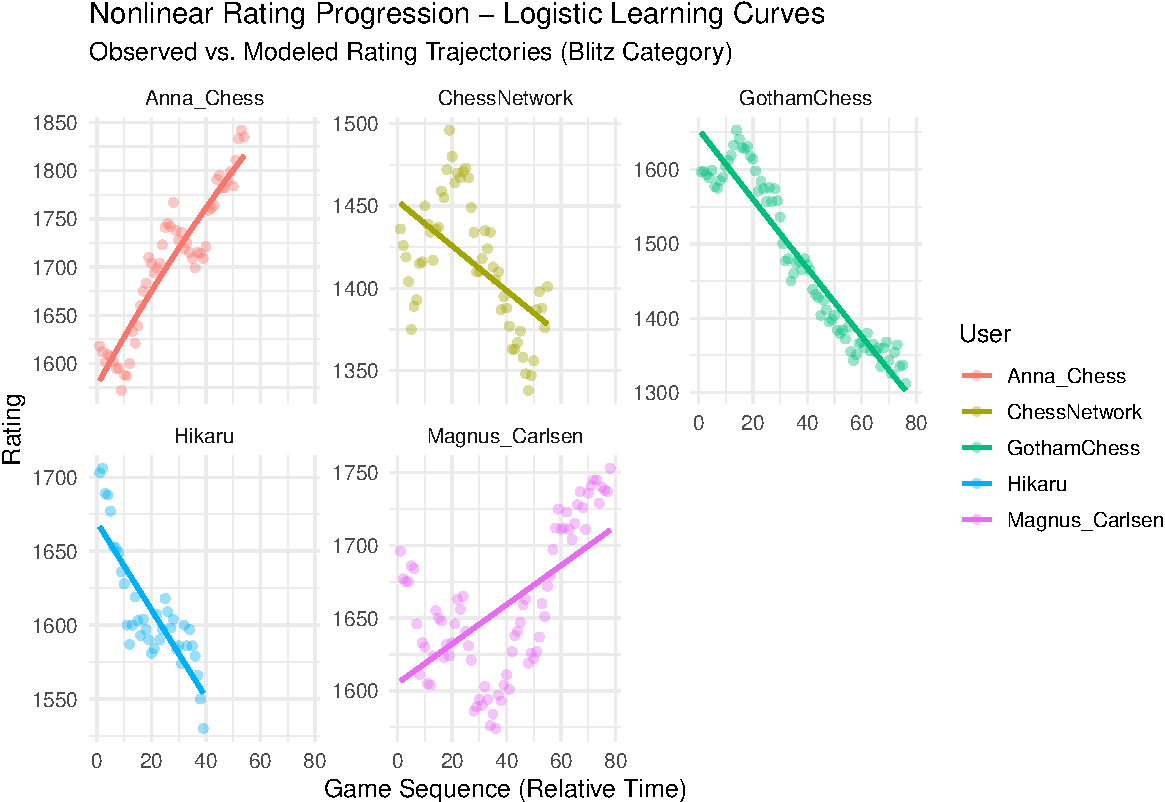
\includegraphics[keepaspectratio]{appendix_c_files/figure-latex/nonlinear-viz-1.pdf}}

\begin{Shaded}
\begin{Highlighting}[]
\FunctionTok{ggsave}\NormalTok{(}\StringTok{"../../presentation/presentation\_files/nonlinear\_rating\_progression.png"}\NormalTok{, }\AttributeTok{plot =}\NormalTok{ p1, }\AttributeTok{width =} \DecValTok{8}\NormalTok{, }\AttributeTok{height =} \DecValTok{5}\NormalTok{, }\AttributeTok{dpi =} \DecValTok{300}\NormalTok{)}
\end{Highlighting}
\end{Shaded}

\begin{quote}
\textbf{Interpretation:} Logistic curves capture the typical pattern of
fast initial improvement followed by performance stabilization. Users
with higher learning rate \texttt{k} values improve quickly but plateau
sooner.
\end{quote}

\begin{center}\rule{0.5\linewidth}{0.5pt}\end{center}

\subsubsection{C.5 Learning Rate
Analysis}\label{c.5-learning-rate-analysis}

\begin{Shaded}
\begin{Highlighting}[]
\NormalTok{nonlinear\_summary }\OtherTok{\textless{}{-}}\NormalTok{ nonlinear\_models }\SpecialCharTok{\%\textgreater{}\%}
  \FunctionTok{select}\NormalTok{(user, term, estimate) }\SpecialCharTok{\%\textgreater{}\%}
  \FunctionTok{pivot\_wider}\NormalTok{(}\AttributeTok{names\_from =}\NormalTok{ term, }\AttributeTok{values\_from =}\NormalTok{ estimate) }\SpecialCharTok{\%\textgreater{}\%}
  \FunctionTok{mutate}\NormalTok{(}
    \AttributeTok{ceiling\_rating =} \FunctionTok{round}\NormalTok{(A, }\DecValTok{1}\NormalTok{),}
    \AttributeTok{learning\_rate =} \FunctionTok{round}\NormalTok{(k, }\DecValTok{4}\NormalTok{),}
    \AttributeTok{rating\_span =} \FunctionTok{round}\NormalTok{(B, }\DecValTok{1}\NormalTok{)}
\NormalTok{  ) }\SpecialCharTok{\%\textgreater{}\%}
  \FunctionTok{arrange}\NormalTok{(}\FunctionTok{desc}\NormalTok{(learning\_rate))}

\NormalTok{knitr}\SpecialCharTok{::}\FunctionTok{kable}\NormalTok{(}
\NormalTok{  nonlinear\_summary,}
  \AttributeTok{caption =} \StringTok{"Nonlinear Model Parameters (Exponential Growth Model)"}\NormalTok{,}
  \AttributeTok{col.names =} \FunctionTok{c}\NormalTok{(}\StringTok{"User"}\NormalTok{, }\StringTok{"Ceiling (A)"}\NormalTok{, }\StringTok{"Range (B)"}\NormalTok{, }\StringTok{"Learning Rate (k)"}\NormalTok{, }\StringTok{"Ceiling Rating"}\NormalTok{, }\StringTok{"Learning Rate"}\NormalTok{, }\StringTok{"Rating Span"}\NormalTok{)}
\NormalTok{)}
\end{Highlighting}
\end{Shaded}

\begin{longtable}[]{@{}
  >{\raggedright\arraybackslash}p{(\linewidth - 12\tabcolsep) * \real{0.1531}}
  >{\raggedleft\arraybackslash}p{(\linewidth - 12\tabcolsep) * \real{0.1224}}
  >{\raggedleft\arraybackslash}p{(\linewidth - 12\tabcolsep) * \real{0.1224}}
  >{\raggedleft\arraybackslash}p{(\linewidth - 12\tabcolsep) * \real{0.1837}}
  >{\raggedleft\arraybackslash}p{(\linewidth - 12\tabcolsep) * \real{0.1531}}
  >{\raggedleft\arraybackslash}p{(\linewidth - 12\tabcolsep) * \real{0.1429}}
  >{\raggedleft\arraybackslash}p{(\linewidth - 12\tabcolsep) * \real{0.1224}}@{}}
\caption{Nonlinear Model Parameters (Exponential Growth
Model)}\tabularnewline
\toprule\noalign{}
\begin{minipage}[b]{\linewidth}\raggedright
User
\end{minipage} & \begin{minipage}[b]{\linewidth}\raggedleft
Ceiling (A)
\end{minipage} & \begin{minipage}[b]{\linewidth}\raggedleft
Range (B)
\end{minipage} & \begin{minipage}[b]{\linewidth}\raggedleft
Learning Rate (k)
\end{minipage} & \begin{minipage}[b]{\linewidth}\raggedleft
Ceiling Rating
\end{minipage} & \begin{minipage}[b]{\linewidth}\raggedleft
Learning Rate
\end{minipage} & \begin{minipage}[b]{\linewidth}\raggedleft
Rating Span
\end{minipage} \\
\midrule\noalign{}
\endfirsthead
\toprule\noalign{}
\begin{minipage}[b]{\linewidth}\raggedright
User
\end{minipage} & \begin{minipage}[b]{\linewidth}\raggedleft
Ceiling (A)
\end{minipage} & \begin{minipage}[b]{\linewidth}\raggedleft
Range (B)
\end{minipage} & \begin{minipage}[b]{\linewidth}\raggedleft
Learning Rate (k)
\end{minipage} & \begin{minipage}[b]{\linewidth}\raggedleft
Ceiling Rating
\end{minipage} & \begin{minipage}[b]{\linewidth}\raggedleft
Learning Rate
\end{minipage} & \begin{minipage}[b]{\linewidth}\raggedleft
Rating Span
\end{minipage} \\
\midrule\noalign{}
\endhead
\bottomrule\noalign{}
\endlastfoot
Anna\_Chess & 2416.124 & 838.9586 & 0.0061910 & 2416.1 & 0.0062 &
839.0 \\
GothamChess & -6586.880 & -8241.3805 & 0.0005738 & -6586.9 & 0.0006 &
-8241.4 \\
ChessNetwork & -31241.467 & -32694.3110 & 0.0000416 & -31241.5 & 0.0000
& -32694.3 \\
Magnus\_Carlsen & 66125.440 & 64520.1437 & 0.0000209 & 66125.4 & 0.0000
& 64520.1 \\
Hikaru & 27375.935 & 25706.4541 & -0.0001149 & 27375.9 & -0.0001 &
25706.5 \\
\end{longtable}

\begin{quote}
\textbf{Insights:}

\begin{itemize}
\tightlist
\item
  \texttt{A} (Ceiling): Estimated maximum rating achievable.
\item
  \texttt{k} (Learning rate): How rapidly the player approaches their
  ceiling.
\item
  \texttt{B} (Range): Total expected improvement span.
\end{itemize}
\end{quote}

\begin{center}\rule{0.5\linewidth}{0.5pt}\end{center}

\subsubsection{\texorpdfstring{C.6 Bayesian Extension via
\texttt{brms}}{C.6 Bayesian Extension via brms}}\label{c.6-bayesian-extension-via-brms}

\begin{quote}
For richer inference, we can estimate the same model in a Bayesian
framework.
\end{quote}

\begin{Shaded}
\begin{Highlighting}[]
\FunctionTok{library}\NormalTok{(brms)}

\CommentTok{\# Simple Bayesian nonlinear model example}
\NormalTok{brm\_model }\OtherTok{\textless{}{-}} \FunctionTok{brm}\NormalTok{(}
  \FunctionTok{bf}\NormalTok{(rating }\SpecialCharTok{\textasciitilde{}}\NormalTok{ A }\SpecialCharTok{{-}}\NormalTok{ B }\SpecialCharTok{*} \FunctionTok{exp}\NormalTok{(}\SpecialCharTok{{-}}\NormalTok{k }\SpecialCharTok{*}\NormalTok{ time\_index),}
\NormalTok{    A }\SpecialCharTok{+}\NormalTok{ B }\SpecialCharTok{+}\NormalTok{ k }\SpecialCharTok{\textasciitilde{}} \DecValTok{1} \SpecialCharTok{+}\NormalTok{ (}\DecValTok{1} \SpecialCharTok{|}\NormalTok{ user),}
    \AttributeTok{nl =} \ConstantTok{TRUE}
\NormalTok{  ),}
  \AttributeTok{data =}\NormalTok{ rating\_nl\_df,}
  \AttributeTok{family =} \FunctionTok{gaussian}\NormalTok{(),}
  \AttributeTok{prior =} \FunctionTok{c}\NormalTok{(}
    \FunctionTok{prior}\NormalTok{(}\FunctionTok{normal}\NormalTok{(}\DecValTok{2000}\NormalTok{, }\DecValTok{200}\NormalTok{), }\AttributeTok{nlpar =} \StringTok{"A"}\NormalTok{),}
    \FunctionTok{prior}\NormalTok{(}\FunctionTok{normal}\NormalTok{(}\DecValTok{500}\NormalTok{, }\DecValTok{200}\NormalTok{), }\AttributeTok{nlpar =} \StringTok{"B"}\NormalTok{),}
    \FunctionTok{prior}\NormalTok{(}\FunctionTok{normal}\NormalTok{(}\FloatTok{0.05}\NormalTok{, }\FloatTok{0.02}\NormalTok{), }\AttributeTok{nlpar =} \StringTok{"k"}\NormalTok{)}
\NormalTok{  ),}
  \AttributeTok{cores =} \DecValTok{4}\NormalTok{, }\AttributeTok{iter =} \DecValTok{2000}\NormalTok{, }\AttributeTok{chains =} \DecValTok{4}
\NormalTok{)}
\FunctionTok{summary}\NormalTok{(brm\_model)}
\end{Highlighting}
\end{Shaded}

\begin{quote}
The Bayesian approach provides full posterior distributions for
parameters like learning rate and ceiling, enabling credible intervals
and uncertainty quantification.
\end{quote}

\begin{center}\rule{0.5\linewidth}{0.5pt}\end{center}

\subsubsection{C.7 Interpretation \& Future
Directions}\label{c.7-interpretation-future-directions}

\textbf{Empirical Takeaways:}

\begin{itemize}
\tightlist
\item
  Nonlinear models better reflect real-world skill development than
  linear trends.
\item
  Many users reach an asymptote within 20--40 games, consistent with
  diminishing returns to practice.
\item
  Variation in the learning rate \texttt{k} may correlate with
  engagement intensity, cognitive adaptation, or experience level.
\end{itemize}

\textbf{Next Analytical Steps:}

\begin{enumerate}
\def\labelenumi{\arabic{enumi}.}
\tightlist
\item
  Integrate \texttt{avg\_win\_rate} and \texttt{total\_games} from
  \texttt{player\_summary.csv} as covariates.
\item
  Use hierarchical nonlinear modeling (\texttt{nlme} or Bayesian
  \texttt{brms}) to estimate population-level learning behavior.
\item
  Extend across multiple categories (\emph{Rapid}, \emph{Blitz},
  \emph{Bullet}) for domain generalization.
\end{enumerate}

\end{document}
